\chapter{Review of Quantum Mechanics}

\section{Spin-1/2 Particle in a Magnetic Field}

The Hamiltonian $H$ for a particle at rest with spin $\vec{S}$ in a magnetic
field $\vec{B}$ is
%
\begin{equation}
H = - \gamma \vec{S} \cdot \vec{B},
\end{equation}
%
where $\gamma$ is the gyromagnetic ratio.
If the magnetic field $\vec{B} = B_{0} \hat{k}$, then
%
\begin{equation}
H = - \gamma B_{0} \vec{S} \cdot \hat{k} = - \gamma B_{0} S_{z}
\end{equation}
%
where $S_{z}$ is the projection of the particles spin along the
z-axis.
%
For spin-1/2 particles
%
\[ S_{z} = \left( \begin{array}{cc}
\frac{\hbar}{2} & 0  \\
0 & -\frac{\hbar}{2} \\
\end{array} \right) = \frac{\hbar}{2} \sigma_{z} ,\]
%
where $\sigma_{z}$ is the Pauli spin matrix
%
\[ \sigma_{z} = \left( \begin{array}{cc}
1 & 0  \\
0 & -1 \\
\end{array} \right) ,\]
%
with eigenvalues $ \lambda_{1,2} = \pm 1$, and corresponding
eigenvectors
\begin{equation}
    \vec{\chi}_{1,2} = 
    \begin{pmatrix}
        1 \\
        0
     \end{pmatrix} ,
    \begin{pmatrix}
        0 \\
        1
    \end{pmatrix}
\end{equation}
which can be relabeled as
\begin{equation}
   \chi_{1} = |\uparrow\rangle = 
    \begin{pmatrix}
        1 \\
        0
     \end{pmatrix} \,\,\, ,  \,\,\,   
    \chi_{2} = |\downarrow\rangle = 
    \begin{pmatrix}
        0 \\
        1
     \end{pmatrix}
\end{equation}
%
The Hamiltonian is then
%
\begin{equation}
  \label{eqn:B0ham}
  H = -\gamma  B_{0} \frac{\hbar}{2}\sigma_{z} = \omega_{0}\frac{\hbar}{2}\sigma_{z} \,\,\, ,
\end{equation}
where $\omega_{0} = \gamma B_{0}$.  The eigenvalues, or energies of
this Hamiltonian are
\begin{equation}
  E_{\uparrow} = -\omega_{0} \frac{\hbar}{2} \,\,\, \textrm{and} \,\,\, E_{\downarrow} = \omega_{0} \frac{\hbar}{2} \,\,\, .
\end{equation}
The corresponding eigenvectors evolve with time as
\begin{equation}
  |\uparrow (t)\rangle = |\uparrow\rangle e^{ -i \frac{E_{\uparrow} t}{\hbar}} = |\uparrow\rangle e^{i \frac{\omega_{0}t}{2}}
\end{equation}
and
\begin{equation}
  |\downarrow (t)\rangle = |\downarrow\rangle e^{ -i \frac{E_{\downarrow} t}{\hbar}} = |\downarrow\rangle e^{-i \frac{\omega_{0}t}{2}}.
\end{equation}
%
The state of the system at time $t$ is

\begin{equation}
  |\psi(t)\rangle = a_{0}|\uparrow(t)\rangle + b_{0}|\downarrow(t)\rangle = \begin{pmatrix}
    a_{0} e^{i \frac{\omega_{0}t}{2}} \\
    b_{0}e^{-i \frac{\omega_{0}t}{2}}
     \end{pmatrix}
\end{equation}
with
\begin{equation}
\label{eqn:psi0}
|\psi(0)\rangle = \begin{pmatrix}
        a_{0} \\
        b_{0}
     \end{pmatrix}.
\end{equation}
%
For normalization, it is require that $|a_{0}|^{2}+|b_{0}|^2 = 1$.  Let
$a_{0} = $cos($\alpha /2$) and $b_{0} = $sin($\alpha /2)$, then

\begin{equation}
  \label{eqn:psi}
  |\psi(t)\rangle = \textrm{cos($\alpha$/2)}|\uparrow\rangle e^{i \frac{\omega_{0}t}{2}} + \textrm{sin($\alpha$/2)}|\downarrow\rangle e^{-i \frac{\omega_{0}t}{2}} = \begin{pmatrix}
    \textrm{cos($\alpha$/2)} e^{i \frac{\omega_{0}t}{2}} \\
    \textrm{sin($\alpha$/2)} e^{-i \frac{\omega_{0}t}{2}}
     \end{pmatrix}.
\end{equation}
This is the time-varying wavefunction of a
spin-1/2 particle in a static magnetic field $\vec{B} = B_{0}\hat{k}$.

\section{Larmor precession\label{sec:Larmor}}

Using Eqn.~\ref{eqn:psi}, we can determine
$\langle S_{x} \rangle$, $\langle S_{y} \rangle$, and
$\langle S_{z} \rangle$, where

\[ S_{x} = \left( \begin{array}{cc}
                    0 & \frac{\hbar}{2}  \\
                    \frac{\hbar}{2} & 0 \\
\end{array} \right) = \frac{\hbar}{2} \sigma_{y} ,\,\,\,\, \textrm{and} \,\,\,\, S_{y} = \left( \begin{array}{cc}
 0 & -i\frac{\hbar}{2}  \\
i\frac{\hbar}{2} & 0 \\
\end{array} \right) = \frac{\hbar}{2} \sigma_{y} ,\]
%
and
%
\begin{equation*}
\langle S \rangle = \langle \psi(t) | S | \psi(t) \rangle .
\end{equation*}

\begin{equation}
\begin{split}
  \langle S_{x} \rangle & =  \begin{pmatrix} \textrm{cos($\alpha$/2)}^{*} e^{-i \frac{\omega_{0}t}{2}} \,\,\, \textrm{sin($\alpha$/2)}^{*} e^{i \frac{\omega_{0}t}{2}} \end{pmatrix}   \begin{pmatrix} 0 & \hbar/2\\ \hbar/2 & 0 \end{pmatrix}  \begin{pmatrix} \textrm{cos($\alpha$/2)} e^{i \frac{\omega_{0}t}{2}}\\ \textrm{sin($\alpha$/2)} e^{-i \frac{\omega_{0}t}{2}} \end{pmatrix}  \\
  & =  \begin{pmatrix} \textrm{cos($\alpha$/2)} e^{-i \frac{\omega_{0}t}{2}} \,\,\, \textrm{sin($\alpha$/2)} e^{i \frac{\omega_{0}t}{2}} \end{pmatrix}  \begin{pmatrix} \frac{\hbar}{2}\textrm{sin($\alpha$/2)} e^{-i \frac{\omega_{0}t}{2}} \\ \frac{\hbar}{2}\textrm{cos($\alpha$/2)} e^{i \frac{\omega_{0}t}{2}} \end{pmatrix}  \\
  & = \frac{\hbar}{2} \textrm{cos($\alpha$/2) sin($\alpha$/2)} e^{-i \omega_{0}t} + \frac{\hbar}{2} \textrm{sin($\alpha$/2) cos($\alpha$/2)} e^{-i \omega_{0}t} \\
  & = \hbar \textrm{cos($\alpha$/2) sin($\alpha$/2)}(\frac{e^{-i \omega_{0}t} + e^{i \omega_{0}t}}{2}) \\
  & = \hbar \textrm{cos($\alpha$/2) sin($\alpha$/2)} \textrm{cos($\omega_{0}$t)} \\
  & = \frac{\hbar}{2}\textrm{sin($\alpha$) cos($\omega_{0}$t)}
\end{split}
\end{equation}

\begin{equation}
\begin{split}
\langle S_{y} \rangle & = \begin{pmatrix} \textrm{cos($\alpha$/2)}^{*} e^{-i \frac{\omega_{0}t}{2}} \,\,\, \textrm{sin($\alpha$/2)}^{*} e^{i \frac{\omega_{0}t}{2}} \end{pmatrix}  \begin{pmatrix} 0 & -i\hbar/2\\ i\hbar/2 & 0 \end{pmatrix}  \begin{pmatrix} \textrm{cos($\alpha$/2)} e^{i \frac{\omega_{0}t}{2}}\\ \textrm{sin($\alpha$/2)} e^{-i \frac{\omega_{0}t}{2}} \end{pmatrix} \\
& =  \begin{pmatrix} \textrm{cos($\alpha$/2)} e^{-i \frac{\omega_{0}t}{2}} \,\,\, \textrm{sin($\alpha$/2)} e^{i \frac{\omega_{0}t}{2}} \end{pmatrix}  \begin{pmatrix} -i\frac{\hbar}{2}\textrm{sin($\alpha$/2)} e^{-i \frac{\omega_{0}t}{2}} \\ i\frac{\hbar}{2}\textrm{cos($\alpha$/2)} e^{i \frac{\omega_{0}t}{2}} \end{pmatrix} \\
& = -i\frac{\hbar}{2} \textrm{cos($\alpha$/2) sin($\alpha$/2)} e^{-i \omega_{0}t} + i\frac{\hbar}{2} \textrm{sin($\alpha$/2) cos($\alpha$/2)} e^{i \omega_{0}t} \\
& = -\hbar \textrm{cos($\alpha$/2) sin($\alpha$/2)}(\frac{e^{i \omega_{0}t} - e^{-i \omega_{0}t}}{2i}) \\
& = -\hbar \textrm{cos($\alpha$/2) sin($\alpha$/2)} \textrm{sin($\omega_{0}$t)} \\
& = -\frac{\hbar}{2}\textrm{sin($\alpha$) sin($\omega_{0}$t)}
\end{split}
\end{equation}

\begin{equation}
\begin{split}
\langle S_{z} \rangle & =  \begin{pmatrix} \textrm{cos($\alpha$/2)}^{*} e^{-i \frac{\omega_{0}t}{2}} \,\,\, \textrm{sin($\alpha$/2)}^{*} e^{i \frac{\omega_{0}t}{2}} \end{pmatrix}  \begin{pmatrix} \hbar/2 & 0\\ 0 & -\hbar/2 \end{pmatrix}\begin{pmatrix} \textrm{cos($\alpha$/2)} e^{i \frac{\omega_{0}t}{2}}\\ \textrm{sin($\alpha$/2)} e^{-i \frac{\omega_{0}t}{2}} \end{pmatrix} \\
& =  \begin{pmatrix} \textrm{cos($\alpha$/2)} e^{-i \frac{\omega_{0}t}{2}} \,\,\, \textrm{sin($\alpha$/2)} e^{i \frac{\omega_{0}t}{2}} \end{pmatrix}  \begin{pmatrix} \frac{\hbar}{2}\textrm{cos($\alpha$/2)} e^{i \frac{\omega_{0}t}{2}} \\ -\frac{\hbar}{2}\textrm{sin($\alpha$/2)} e^{-i \frac{\omega_{0}t}{2}} \end{pmatrix}  \\
& = \frac{\hbar}{2}(\textrm{cos$^{2}(\alpha/2)$ - sin$^{2}(\alpha/2)$}) \\
& = \frac{\hbar}{2}(\textrm{cos$^{2}(\alpha/2)$ - 1+ cos$^{2}(\alpha/2)$}) \\
& = \frac{\hbar}{2}(2\textrm{cos($\alpha/2)^{2}$ - 1}) \\
& = \frac{\hbar}{2}(2\left(\frac{1 + \textrm{cos($\alpha$)}}{2}\right) - 1) \\
& = \frac{\hbar}{2}\textrm{cos($\alpha$)}
\end{split}
\end{equation}

\section{Effect of RF Pulses and NMR Lineshape\label{sec:rfpulse}}
In this section the effect of adding an oscillating field at
resonance, perpendicular to the static $B_0$ field is studied. Consider
%
\begin{equation}
\begin{split}
&\vec{B}_{0} = B_{0} \hat{z}, \;\;\;\;\;\;
\vec{B}_{1} = B_{1}\textrm{cos}(\omega t) \hat{i} - B_{1} \textrm{sin} (\omega t) \hat{j} \\
%
&\vec{B} = \vec{B}_{0} + \vec{B}_{1} = B_{0}\hat{z} + B_{1}(\textrm{cos}(\omega t) \hat{i} - \textrm{sin}(\omega t) \hat{j}).
\end{split}
\end{equation}
The Hamiltonian would be
\begin{equation}
\begin{split}
H= -\vec{\mu}\cdot \vec{B} = -\gamma \vec{S} \cdot \vec{B} 
& = -\gamma(B_{0}S_{z} + B_{1}\textrm{cos}(\omega t)S_{x} - B_{1}\textrm{sin}(\omega t)S_{y}) \\
& = -\gamma \frac{\hbar}{2}(B_{0}\sigma_{z} + B_{1}\textrm{cos}(\omega t)\sigma_{x} - B_{1}\textrm{sin}(\omega t)\sigma_{y}).
\end{split}
\end{equation}

%\begin{equation}
%\hat{H}  = -\gamma\frac{\hbar}{2} \left(\begin{pmatrix} %B_{0} & 0 \\ 0 & -B_{0} \end{pmatrix} + \begin{pmatrix} 0 & %B_1 \textrm{cos}(\omega t) \\ B_1 \textrm{cos}(\omega t) & %0 \end{pmatrix} - i \begin{pmatrix} 0 & %-B_{1}\textrm{sin}(\omega t) \\ B_{1}\textrm{sin}(\omega t) %& 0 \end{pmatrix}\right)
%\end{equation}
In matrix form
\begin{equation}
\begin{split}
  H &= -\gamma \frac{\hbar}{2} \begin{pmatrix} B_{0} & B_{1}(\textrm{cos}(\omega t) + i\textrm{sin}(\omega t)) \\ B_{1}(\textrm{cos}(\omega t) - i\textrm{sin}(\omega t)) & -B_{0} \end{pmatrix} \\
%
&= -\gamma \frac{\hbar}{2} \begin{pmatrix} B_{0} & B_{1} e^{i\omega t} \\ B_{1}e^{-i\omega t} & -B_{0} \end{pmatrix}.
\end{split}
\end{equation}

The Schr\"{o}dinger equation
\begin{equation}
H|\psi(t) \rangle = i\hbar\frac{\partial}{\partial t}|\psi(t) \rangle
\end{equation}
would then become        
\begin{equation}
-\gamma \frac{\hbar}{2}\begin{pmatrix} B_{0} & B_{1}e^{i\omega t} \\ B_{1}e^{-i\omega t} & -B_{0} \end{pmatrix} \begin{pmatrix} a(t) \\ b(t) \end{pmatrix} = i\hbar\frac{\partial}{\partial t} \begin{pmatrix} a(t) \\ b(t) \end{pmatrix}.
\end{equation} 
\\
This gives two coupled differential equations to solve.  Letting
$\gamma B_{0} = \omega_{0}$, and $\gamma B_{1} = \omega_{1}$, then

\begin{equation}
\label{eqn:adot}
%i\hbar\frac{\partial a(t)}{\partial t} = -\frac{\hbar}{2} \left[\omega_{0} a(t) + \omega_{1}e^{i\omega t}b(t)\right] \;\;\; \textrm{or} \;\;\; 
\dot{a}(t) = \frac{i}{2}[\omega_{0}a(t)+\omega_{1}e^{i\omega t}b(t)].
\end{equation}
%
and
%
\begin{equation}
\label{eqn:bdot}
%i\hbar\frac{\partial a(t)}{\partial t} = -\frac{\hbar}{2} \left[\omega_{1} e^{-i\omega t}a(t) - \omega_{0}b(t)\right] \;\;\; \textrm{or} \;\;\; 
\dot{b}(t) = \frac{i}{2}[\omega_{1}e^{-i\omega t}a(t)-\omega_{0}b(t)].
\end{equation}
%
Eqn.~\ref{eqn:adot} and Eqn.~\ref{eqn:bdot} could be solved by taking
the second order derivative of $a(t)$
%
\begin{equation}
\label{eqn:addot}
\ddot{a} = \frac{i}{2}(\omega_{0}\dot{a}+i\omega \omega_{1} e^{i\omega t} b + \omega_{1}e^{i\omega t} \dot{b})  .
\end{equation}
%
Using Eqn.~\ref{eqn:adot} and solving for $b$ in terms of $a$
and $\dot{a}$
%
\begin{equation}
\label{eqn:b}
b = \frac{-i 2 \dot{a} - \omega_{0} a}{\omega_{1}}e^{-i\omega t} .
\end{equation}
%
Plugging Eqn.~\ref{eqn:bdot} and Eqn.~\ref{eqn:b} into
Eqn.~\ref{eqn:addot} gives
%
\begin{equation}
\label{eqn:diffeqn}
\ddot{a} = i\omega \dot{a} - \frac{a}{4} (\omega^{2} + \omega_{0}^{2} - 2\omega\omega_{0}) ~ ,
\end{equation}
%
which has a solution of the form $a = a_{0}e^{i\alpha t}$, where
$a_{0}$ and $\alpha$ are parameters to be determined.  Plugging this
into Eqn.~\ref{eqn:diffeqn} gives
%
\begin{equation}
0 = \alpha^{2} - \omega \alpha - \frac{\omega_{1}^{2} + \omega_{0}^{2} - 2\omega \omega_{0}}{4} 
\end{equation}
%
and therefore
%
\begin{equation}
\alpha_{\pm} = \frac{\omega \pm \omega'}{2} , \;\;\;  \omega' = \sqrt{\omega_{1}^{2} + (\omega_{0}-\omega)^{2}}  .
\end{equation}
%
General solution of $a(t)$ could be written as
%We can construct a general solution for $a(t)$ using the two solutions
%of $\alpha$:
%
\begin{equation}
\label{eqn:gena}
a(t)=c_{1}e^{i\alpha_{+}t} + c_{2}e^{i\alpha_{-}t} \;\; ,
\end{equation}
%
where $c_{1}$ and $c_{2}$ are constants to be determined from initial
conditions.  Plugging Eqn.~\ref{eqn:gena}, and it's first order
time-derivative into Eqn.~\ref{eqn:b} gives the general solution for
$b(t)$
%
\begin{equation}
b(t) = \frac{1}{\omega_{1}}[c_{1}(2\alpha_{+}-\omega_{0})e^{i\alpha_{+}t} + c_{2}(2\alpha_{-}-\omega_{0})e^{i\alpha_{-}t}]e^{-i\omega t}.
\end{equation}
%
At $t=0$, the solutions of $a(t)$ and $b(t)$ become
%
\begin{equation}
\begin{split}
& a(0)= a_{0} = c_{1} + c_{2} \\
& b(0) = b_{0} = \frac{1}{\omega_{1}}[c_{1}(2\alpha_{+}-\omega_{0}+ c_{2}(2\alpha_{-}-\omega_{0}))].
\end{split}
\end{equation}
%
Solving for $c_{1}$ and $c_{2}$ in terms of $a_{0}$ and $b_{0}$ gives
%
\begin{equation}
\begin{split}
&c_{1} = a_{0}(\frac{\omega' - \omega + \omega_{0}}{2\omega'}) + \frac{\omega_{1}b_{0}}{2\omega'} \\
&c_{2} = \frac{1}{\omega'}[a_{0}(\omega+\omega'-\omega_{0})-\omega_{1}b_{0}].
\end{split}
\end{equation}
%
Plugging $c_{1}$ and $c_{2}$ into the general solutions of $a(t)$ and
$b(t)$ gives
%
\begin{equation}
\begin{split}
&a(t) = \left\lbrace a_{0} \textrm{cos}(\omega' t/2) + \frac{i}{\omega'}[a_{0}(\omega_{0}-\omega) + b_{0}\omega_{1}] \textrm{sin}(\omega' t/2)
\right\rbrace e^{\frac{i\omega t}{2}} \\
&b(t) = \left\lbrace b_{0} \textrm{cos}(\omega' t/2) + \frac{i}{\omega'}[b_{0}(\omega-\omega_{0}) + a_{0}\omega_{1}]\textrm{sin}(\omega' t/2) \right\rbrace e^{\frac{-i\omega t}{2}}.
\end{split}
\end{equation}
%
If the particle starts out at $t=0$ with spin up ({\it i.e}., $a_{0} =1$,
$b_{0} = 0$),
%
\begin{equation}
\begin{split}
&a(t) =  \left\lbrace \textrm{cos}(\omega' t/2) + \frac{i}{\omega'}(\omega_{0}-\omega)\textrm{sin}(\omega' t/2)
\right\rbrace e^{\frac{i\omega t}{2}} \\
&b(t) = \frac{i}{\omega'}\textrm{sin}(\omega' t/2) e^{\frac{-i\omega t}{2}}
\end{split}
\end{equation}
%
and the probability of a transition to spin down, as a function of
time, is then
%
\begin{equation}
\begin{split}
P(t) &= |b(t)|^2 \\
&= |\frac{-i}{\omega'}\textrm{sin}(\omega' t/2) e^{\frac{i\omega t}{2}}||\frac{i}{\omega'}\textrm{sin}(\omega' t/2) e^{\frac{-i\omega t}{2}}| \\
&=\frac{\omega_1^2}{\omega'^2}\textrm{sin}^{2}(\frac{\omega' t}{2}) \\
&=\frac{\omega_1^2}{\omega_{1}^2 + (\omega_0 - \omega)^2}\textrm{sin}^{2}(\frac{\omega' t}{2}) \\
&=\frac{\omega_1^2}{\omega_{1}^2 + (\omega_0 - \omega)^2}\frac{1- \textrm{cos}(\omega' t)}{2}.
\end{split}
\end{equation}
%
A maximum will occur on resonance when $\omega = \omega_0$, and when
$\omega ' t = \pi$. Then for $\omega'$ would become
%
\begin{equation}
\begin{split}
\omega' &= \sqrt{\omega_{1}^{2} + (\omega_{0}-\omega)^{2}} \\
& = \sqrt{\omega_{1}^{2} + (\omega_{0}-\omega_0)^{2}} \\
& = \omega_{1} \;\;\; ,
\end{split}
\end{equation}
%
which gives a pulse length of
\begin{equation}
t = \frac{\pi}{\omega'} =\frac{\pi}{\omega_1} \;\; .
\end{equation}
%
Defining a dimensionless parameter $x = (\frac{\omega_0 - \omega}{\omega_1})^2$, and setting $\omega_1 t = \pi$ gives
%
\begin{equation}
P(x)=\frac{1}{1 + x^2}\textrm{sin}^{2}(\sqrt{(x^2 +1)}\frac{\pi}{2}).
\end{equation}

\begin{figure}[h!]
  \centering 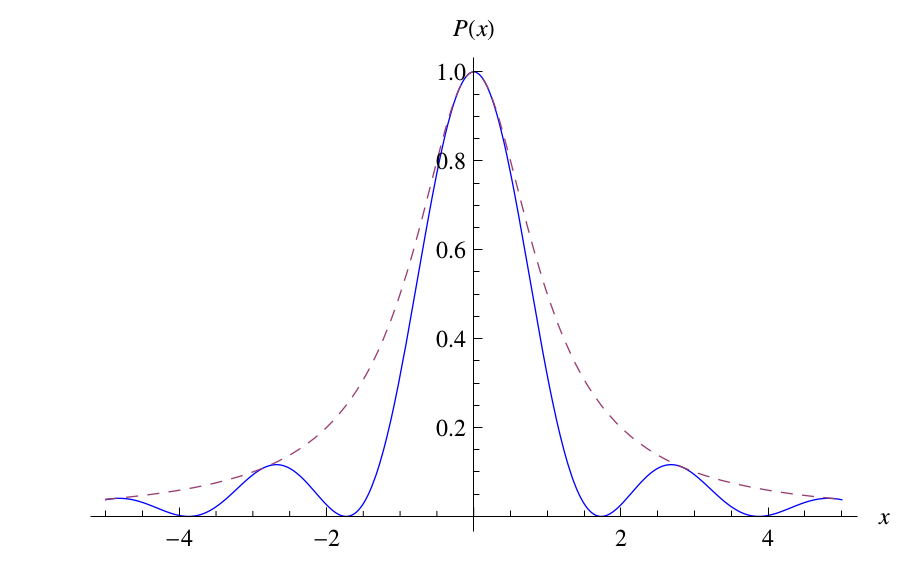
\includegraphics[width=1\textwidth]{NMR_Lineshape.png}
  \caption{The solid blue line shows the probability of the transition
    from spin-up to spin-down with $\omega_1 t = \pi$.  The dashed
    line shows the envelope of the transition probability, which is
    the simply 1/(1+x$^2$).}
    \label{fig:trans}
\end{figure} 
%
It is clear from Fig. \ref{fig:trans} that the probability of a
transition from spin-up to spin-down is most likely to occur when
$x=0$, which corresponds to $\omega = \omega_0$.  $\omega_0$ is then
considered to be the resonant frequency of this system, and is known
as the Larmor precession frequency.
